\documentclass[12pt]{amsart}

\usepackage{stmaryrd}
\usepackage{enumerate}
\usepackage{epsfig}

\begin{document} 

\newtheorem{theorem}{Theorem}
\newtheorem{proposition}{Proposition}
\newtheorem{lemma}{Lemma}
\newtheorem{corollary}{Corollary}
\newtheorem{definition}{Definition}
\newenvironment{remark}{\medskip\noindent{\textbf{Remark.}}}{\medskip}
\newenvironment{bibremark}{\begin{footnotesize}\medskip\noindent{\textbf{Bibliographic remark.}}}{\end{footnotesize}\medskip}

\makeatletter
\newlength{\earraycolsep}
\setlength{\earraycolsep}{2pt}
\def\eqnarray{\stepcounter{equation}\let\@currentlabel%
\theequation
\global\@eqnswtrue\m@th
\global\@eqcnt\z@\tabskip\@centering\let\\\@eqncr
$$\halign to\displaywidth\bgroup\@eqnsel\hskip\@centering
$\displaystyle\tabskip\z@{##}$&\global\@eqcnt\@ne
\hskip 2\earraycolsep \hfil$\displaystyle{##}$\hfil
&\global\@eqcnt\tw@ \hskip 2\earraycolsep
$\displaystyle\tabskip\z@{##}$\hfil
\tabskip\@centering&\llap{##}\tabskip\z@\cr}
\makeatother

\title{Stars in multi-triangulations}

\begin{abstract}
\end{abstract}

\maketitle

\section{Introduction}

IN PROGRESS





\section{Notation}

Let $k$ and $n$ be two integers such that $k\ge 1$ and $n\ge 2k+1$.

Let $\mathbb{Z}_n$ denote the cyclic set $\{i+n\mathbb{Z}\;|\; 0\le i\le n-1\}$.
Let $V_n=\{v_i\;|\; i\in\mathbb{Z}_n\}$ be a set of $n$ distinct points of the unit circle, labelled by $\mathbb{Z}_n$ counterclockwise.
The set $V_n$ is identified with any other such set and is named the \emph{set of vertices of the $n$-gon}.
It inherits the \emph{cyclic order} from $\mathbb{Z}_n$ and for $u,v,w\in V_n$, we will denote this order $u
\le v\le w$.
For any $u,v\in V_n$, let $\llbracket u,v\rrbracket$ (resp. $\rrbracket u,v\llbracket$) denote the \emph{cyclic interval} $\{w\in V_n\;|\; u\le w\le v\}$ (resp. $\{w\in V_n\;|\; u<w<v\}$).

For $\{i,j\}\in{\mathbb{Z}_n \choose 2}$, let $e_{ij}=[v_i,v_j]$ denote the \emph{edge} connecting the vertices $v_i$ and $v_j$. The set $E_n=\{e_{ij}\;|\; \{i,j\}\in{\mathbb{Z}_n \choose 2}\}$ is the \emph{set of edges of the $n$-gon}.
Two edges $e_{ij}$ and $e_{i'j'}$ are said to be \emph{intersecting} when the intersection $]v_i,v_j[\cap]v_{i'},v_{j'}[$ is non-empty.
For $\ell\in\mathbb{N}$, an \emph{$\ell$-crossing} is a set of $\ell$ mutually intersecting edges of $E_n$.

A \emph{$k$-triangulation} of the $n$-gon is a maximal subset of $E_n$ which does not contain any $(k+1)$-crossing.

Obviously, an edge $e_{ij}$ of $E_n$ can appear in a $(k+1)$-crossing only if $|i-j|>k$. Such an edge is said to be \emph{$k$-relevant}. An edge $e_{ij}$ is said to be \emph{$k$-almost-relevant} if $|i-j|=k$ and \emph{$k$-irrelevant} if $|i-j|<k$.
Every $k$-triangulation of the $n$-gon contains all the $(k-1)n$ $k$-irrelevant edges and all the $n$ $k$-almost-relevant edges of the $n$-gon and some $k$-relevant edges.

A \emph{$k$-star} of the $n$-gon is a set $S=\{[s_j,s_{j+k}]\;|\; j\in\mathbb{Z}_{2k+1}\}$ of $2k+1$ edges of $E_n$ where $\{s_j\;|\; j\in\mathbb{Z}_{2k+1}\}$ are $2k+1$ vertices cyclically labelled by $\mathbb{Z}_{2k+1}$. The set $\{s_j\;|\; j\in\mathbb{Z}_{2k+1}\}$ is the set of vertices of $S$ and is denoted $V(S)$. Note that there are two natural cyclic orders on $V(S)$: the \emph{circle order}, defined as the cyclic order around the circle, and the \emph{star order}, defined as the cyclic order tracing the edges of $S$. More precisely, if $s_0,\ldots,s_{2k}$ are the vertices of $S$ cyclically ordered around the circle, we rename the vertices $r_i=s_{ki}$ to obtain the star order $r_0,\ldots,r_{2k}$ (see fig. \ref{star}).

\begin{figure}
\centerline{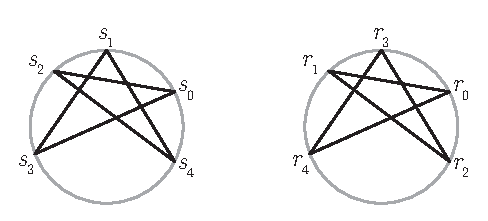
\includegraphics[scale=1]{star.eps}}
\caption{\small{The two cyclic orders on the vertices of a $2$-star: the circle order (left) and the star order (right).}}\label{star}
\end{figure}

An \emph{angle} of a subset $F$ of $E_n$ is a pair of edges $\widehat{xyz}=\{[x,y],[y,z]\}$ of $F$ such that $x<y<z<x$ and for all $t\in\rrbracket z,x\llbracket$, $[y,t]\notin F$. The vertex $y$ is the \emph{vertex of the angle} $\widehat{xyz}$. We say that an angle $\widehat{xyz}$ looks at a vertex $t$ if $t\in\rrbracket z,x\llbracket$. An angle is said to be \emph{$k$-relevant} if its edges are either $k$-relevant or $k$-almost-relevant. 

\section{Star-edge incidence}

\begin{lemma}\label{starcaracterization}
Let $T$ be a $k$-triangulation and let $s_0,\ldots,s_{2k}$ be the vertices of a $k$-star in star order. Then for every $i\in\mathbb{Z}_{2k+1}$, $\widehat{s_{i}s_{i+1}s_{i+2}}$ is a $k$-relevant angle of $T$.
\end{lemma}

\begin{proof}
Suppose that $T$ contains an edge $[s_{i+1},t]$ where $t\in\rrbracket s_{i+2},s_i\llbracket$. Then the set of edges $$[s_{i+2},s_{i+3}],[s_{i+4},s_{i+5}],\ldots,[s_{i-1},s_{i}],[s_{i+1},t]$$ forms a $(k+1)$-crossing. Since any edge of a $k$-star $S$ has $k$ points  of $S$ on one side and $k-1$ on the other side, it is $k$-relevant or $k$-almost-relevant, so that $\widehat{s_{i}s_{i+1}s_{i+2}}$ is a $k$-relevant angle of $T$.
\end{proof}

\begin{theorem}\label{angle}
Any $k$-relevant angle of a $k$-triangulation $T$ is contained in a unique $k$-star of $T$.
\end{theorem}

In order to prove this theorem, we need the following definition: if $\widehat{uvw}$ is a $k$-relevant angle of a $k$-triangulation $T$ and if $[a,b]$ and $[c,d]$ are two edges of $T$ such that $u<a<v<b<w$ and $u<c<v<d<w$ (for the cyclic order), then we will say that $[a,b]$ is \emph{$\widehat{uvw}$-farther} than $[c,d]$ if $u<a\le c<v<d\le b<w$. If $E$ and $F$ are two $(k-1)$-crossings with respective edges $e_1=[a_1,b_1],e_2=[a_2,b_2],\ldots,e_{k-1}=[a_{k-1},b_{k-1}]$ and $f_1=[c_1,d_1],f_2=[c_2,d_2],\ldots,f_{k-1}=[c_{k-1},d_{k-1}]$ such that $u<a_1<a_2<\ldots<a_{k-1}<v<b_1<b_2<\ldots<b_{k-1}<w$ and $u<c_1<c_2<\ldots<c_{k-1}<v<d_1<d_2<\ldots<d_{k-1}<w$, then we will say that $E$ is \emph{$\widehat{uvw}$-farther} than $F$ if $e_i$ is $\widehat{uvw}$-farther than $f_i$ for every $1\le i\le k-1$. We will say that a $(k-1)$-crossing $E$ is \emph{$\widehat{uvw}$-maximal} if there does not exist any $k$-crossing $\widehat{uvw}$-farther than $E$.


\begin{proof}[Proof of theorem \ref{angle}]
Let $T$ be a $k$-triangulation, and let $\widehat{uvw}$ be a $k$-relevant angle of $T$. 
Suppose first that the edge $[u,v+1]$ is not in $T$. Thus we have a $k$-crossing $E$ of the form $e_1=[a_1,b_1],\ldots,e_k=[a_k,b_k]$ with $u<a_1<\ldots<a_k<v+1$ and $v+1<b_1<\ldots<b_k<u$. Since $[u,v]\in T$, $a_k=v$ and since $\widehat{uvw}$ is an angle, $v+1<b_k\le w$. Consequently, $u<a_1<\ldots<a_{k-1}<v<b_1<\ldots<b_{k-1}<w$ and we can assume that the set $\{e_1,\ldots,e_{k-1}\}$ forms a $(k-1)$-crossing $\widehat{uvw}$-maximal. We will prove that the edges $[u,b_1], [a_1,b_2],\ldots, [a_{k-2},b_{k-1}],[a_{k-1},w]$ are edges of $T$ and this will prove that the points $u$, $a_1,\ldots,a_{k-1}$, $v$, $b_1,\ldots,b_{k-1}$, $w$ are the vertices of a $k$-star of $T$. To get this result, we use two steps: first we prove that $\{[a_1,b_1],[b_1,u]\}$ is an angle of $T$, and then we prove that the edges $e_2,\ldots,e_{k-1},[v,w]$ form a $(k-1)$-crossing $\widehat{a_1b_1u}$-maximal (so that we can reiterate the argument).

\medskip
\noindent\textsc{First step.}
Suppose that $[u,b_1]$ is not in $T$. Thus we have a $k$-crossing $F$ that prevents the edge $[u,b_1]$. Let $f_1=[c_1,d_1],\ldots,f_k=[c_k,d_k]$ denote its edges with $u<c_1<\ldots<c_k<b_1$ and $b_1<d_1<\ldots<d_k<u$.

Note first that $d_k\le w$. Indeed, if it is not the case, then $d_k\in\rrbracket w,u\llbracket$ and $c_k\ne v$, because $\widehat{uvw}$ is an angle. Thus either $c_k\in\rrbracket u,v\llbracket$ and  then $F\cup\{[u,v]\}$ forms a $(k+1)$-crossing, or $c_k\in\rrbracket v,b_1\llbracket$ and  then $E\cup\{[c_k,d_k]\}$ forms a $(k+1)$-crossing. Consequently, we have $b_1<d_1<\ldots<d_{k-1}<w$.

Let $\ell=\max\{1\le i\le {k-1}\;|\; b_i< d_i<w\}$. Then for any $1\le i\le\ell$, since $\{e_1,\ldots,e_i\}\cup\{f_i,\ldots,f_k\}$ does not form a $(k+1)$-crossing, we have $u<c_i\le a_i$. Thus for any $1\le i\le\ell$, $u<c_i\le a_i<v<b_i<d_i<w$, so that $f_i$ is $\widehat{uvw}$-farther than $e_i$. Furthermore, we have $u<c_1<\ldots<c_\ell< a_{\ell+1}<\ldots<a_{k-1}<v<d_1<\ldots<d_\ell<b_{\ell+1}<\ldots<b_{k-1}<w$. Consequently, we get a $(k-1)$-crossing $\{f_1,\ldots,f_\ell,e_{\ell+1},\ldots,e_{k-1}\}$ which is $\widehat{uvw}$-farther than $\{e_1,\ldots,e_{k-1}\}$ which is a contradiction with the definition of $\{e_1,\ldots,e_{k-1}\}$. Thus we obtain $[u,b_1]\in T$.

Suppose now that $\{[a_1,b_1],[b_1,u]\}$ is not an angle of $T$ then there exists $a_0\in \rrbracket u,a_1\llbracket$ such that $[b_1,a_0]\in T$. But then the $(k-1)$-crossing $\{[a_0,b_1],e_2,\ldots,e_{k-1}\}$ is $\widehat{uvw}$-farther than $\{e_1,\ldots,e_{k-1}\}$, so that $\widehat{a_1b_1u}$ is an angle of $T$.

\medskip
\noindent\textsc{Second step.}
Let $F$ be a $(k-1)$-crossing $\widehat{a_1b_1u}$-farther than the $(k-1)$-crossing $\{e_2,\ldots,e_{k-1},[v,w]\}$. Let $f_2=[c_2,d_2],\ldots,f_k=[c_k,d_k]$ denote its edges such that $a_1<c_2<\ldots<c_k<b_1<d_2<\ldots<d_k<u$. 

Note first that $d_k\le w$. Indeed, if it is not the case, then $d_k\in\rrbracket w,u\llbracket$ and $c_k\ne v$, because $\widehat{uvw}$ is an angle. Thus either $c_k\in\rrbracket a_1,v\llbracket$ and  then $F\cup\{[u,v],e_1\}$ forms a $(k+1)$-crossing, or $c_k\in\rrbracket v,b_1\llbracket$ and  then $E\cup\{[c_k,d_k]\}$ forms a $(k+1)$-crossing. Consequently, we have $b_1<d_2<\ldots<d_{k-1}<w$.

Furthermore, for any $2\le i\le k-1$, $f_i$ is $\widehat{a_1b_1u}$-farther than $e_i$, so that $a_1<c_i\le a_i<b_1<b_i\le d_i<u$. In particular, $a_1<c_{k-1}\le a_{k-1}<v$ and we get $u<a_1<c_2<\ldots<c_{k-1}<v<b_1<d_2<\ldots<d_{k-1}<w$. Consequently, the $(k-1)$-crossing $\{e_1,f_2,\ldots,f_{k-1}\}$ is $\widehat{uvw}$-farther than $\{e_1,\ldots,e_{k-1}\}$, which is a contradiction. This finishes the proof when the edge $[u,v+1]$ is not in $T$.

\medskip
Suppose now that $[u,v+1]$ is in $T$. Then
\begin{enumerate}[(i)]
\item either there exists $1\le\ell\le 2k-1$ such that
$$\{[u+\lfloor i/2\rfloor,v+\lceil i/2\rceil]\;|\; 0\le i\le \ell\}\subset T$$
$$\mathrm{and}\; [u+\lfloor (\ell+1)/2\rfloor,v+\lceil (\ell+1)/2\rceil]\notin T.$$
Suppose for instance that $\ell$ is even (when $\ell$ is odd, the argument is similar). Let $u'=u+\ell/2$, $v'=v+\ell/2$ and $w'=u+\ell/2-1$. Then $\widehat{u'v'w'}$ is an angle of $T$ and $[u',v'+1]\notin T$, so that there exists a $k$-star $S$ containing $\widehat{u'v'w'}$. Then the previous lemma ensures that $S$ contains $\widehat{uvw}$.
\item or $\{[u+\lfloor i/2\rfloor,v+\lceil i/2\rceil]\;|\; 0\le i\le 2k\}\subset T$.
But then, in order not to form a $(k+1)$-crossing, we have $n=2k+1$, $T=E_n$ and any $k$-relevant angle of $T$ is contained in the $k$-star with vertices $V_n$.
\end{enumerate}

\medskip
We obtain that any $k$-relevant angle of $T$ is contained in at least one $k$-star of $T$, and the previous lemma ensures the uniqueness of this $k$-star.
\end{proof}

\begin{corollary}\label{incidences}
Let $T$ be a $k$-triangulation. Every $k$-relevant edge belongs to exactly two $k$-stars of $T$ (one on each side), every $k$-almost-relevant edge belongs to one $k$-star of $T$ (on the interior side) and every $k$-irrelevant edge does not belong to any $k$-star of $T$.
\end{corollary}

\begin{corollary}\label{commonedges}
Two distinct $k$-stars $R$ and $S$ of a $k$-triangulation can not share two edges that are consecutive for the star order. In particular, $R$ and $S$ can not share more than $k$ edges.
\end{corollary}


\section{Opposite vertices}

\begin{lemma}
Let $A=\{a_i\;|\; i\in\mathbb{Z}_{2k+1}\}$ and $B=\{b_j\;|\; j\in\mathbb{Z}_{2k+1}\}$ be two distinct sets of $2k+1$ points of the unit circle, labelled in star order, such that for any $i,j\in\mathbb{Z}_{2k+1}$,
\begin{enumerate}
\item if $a_i\in\rrbracket b_{j+1},b_{j-1}\llbracket$, then $b_j\notin\{a_{i+1},a_{i-1}\}$,
\item if $b_j\in\rrbracket a_{i+1},a_{i-1}\llbracket$, then $a_i\notin\{b_{j+1},b_{j-1}\}$.
\end{enumerate}
Then there exists $i,j\in\mathbb{Z}_{2k+1}$ such that $a_i\in\rrbracket b_{j+1},b_{j-1}\llbracket$ and $b_j\in\rrbracket a_{i+1},a_{i-1}\llbracket$
\end{lemma}

\begin{proof}
IN PROGRESS
\end{proof}

\begin{theorem}\label{oppositevertices}
For any two $k$-stars $R$ and $S$ in a $k$-triangulation there are unique distinguished \emph{opposite vertices} $r_0$ and $s_0$ such that if $r_0,\dots,r_{2k}$ and $s_0,\dots, s_{2k}$ are the vertices of $R$ and $S$, in star order, then $r_0\in\rrbracket s_1,s_{2k}\llbracket$ and $s_0\in\rrbracket r_1,r_{2k}\llbracket$ (ie. the angles $\widehat{s_{2k}s_0s_1}$ and $\widehat{r_{2k}r_0r_1}$ look at $r_0$ and $s_0$ respectively).

Moreover, for every $1\le i\le k$, $r_{2i-1}\in\rrbracket r_0,s_{2i}\rrbracket$ and $s_{2i-1}\in\rrbracket s_0,r_{2i}\rrbracket$.
In particular, for every $i\in\mathbb{Z}_{2k+1}$ the edges $[r_i,r_{i+1}]$ and $[s_i,s_{i+1}]$ do not cross.
\end{theorem}

\begin{figure}
\centerline{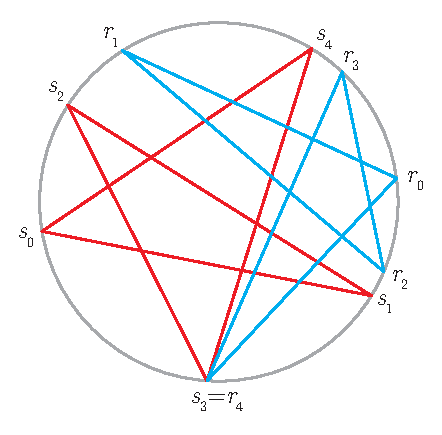
\includegraphics[scale=1]{oppvert.eps}}
\caption{\small{The two opposite vertices of two $2$-stars.}}\label{oppvert}
\end{figure}


\begin{proof}
The previous lemma ensures the existence of such a couple.

Let $r_0,\ldots,r_{2k}$ and $s_0,\ldots,s_{2k}$ be the vertices of $R$ and $S$, in star order, and suppose that $r_0\in\rrbracket s_1,s_{2k}\llbracket$ and $s_0\in\rrbracket r_1,r_{2k}\llbracket$. Furthermore, suppose that there exists $(a,b)\in(\mathbb{Z}_{2k+1})^2\setminus\{(0,0)\}$ such that $r_a\in\rrbracket s_{b+1},s_{b-1}\llbracket$ and $s_b\in\rrbracket r_{a+1},r_{a-1}\llbracket$. Note that certainly, $a\ne0$, $b\ne0$, and $a$ and $b$ have the same parity. By symmetry, we can assume that $a=2\alpha$, $b=2\beta$ with $1\le\beta\le\alpha\le k$. But then the set
$$\{[r_{2i},r_{2i+1}]\;|\; 0\le i\le \alpha-1\}\cup\{[s_{2j},s_{2j+1}]\;|\; \beta\le j\le k\}$$
forms a $(k+1+\alpha-\beta)$-crossing, and $k+1+\alpha-\beta\ge k+1$. This proves that such a couple is unique.

Assume now that there exists $1\le i\le k$ such that $r_{2i-1}\in\rrbracket s_{2i},s_0\llbracket$ or $s_{2i-1}\in\rrbracket r_{2i},r_0\llbracket$. Let $\gamma$ be the highest such integer, and assume for example that $r_{2\gamma-1}\in\rrbracket s_{2\gamma},s_0\llbracket$. Then the definition of $\gamma$ ensures that
$s_0<s_{2\gamma+1}\le r_{2\gamma}<r_{2\gamma-2}$
so that the set
$$\{[r_{2i},r_{2i+1}]\;|\; 0\le i\le\gamma-1\}\cup\{[s_{2j},s_{2j+1}]\;|\; \gamma\le j\le k\}$$
forms a $(k+1)$-crossing.

The last point is now a direct consequence.
\end{proof}

%\begin{remark}
%Another proof, more geometric, would be to assume that the vertices of the $k$-star $R$ are regularily distributed on the unit circle. Then $s_0$ will be the unique vertex of $S$ such that if $s_0,\dots, s_{2k}$ are the vertices of $S$, in star order, then the origine of the plane is contained in the angle $\widehat{s_{2k}s_0s_1}$. And $r_0$ will be the unique vertex of $R$ such that if $r_0,\dots,r_{2k}$ are the vertices of $R$, in star order, $s_0\in\rrbracket r_1,r_{2k}\llbracket$.
%\end{remark}

\begin{lemma}\label{findingstars}
Let $T$ be a $k$-triangulation.
\begin{enumerate}
\item For any $k$-star $S$ of $T$ and for any vertex $r$ not in $S$ there is a unique $k$-star $R$ of $T$ such that $r$ is the vertex of $R$ opposite to $S$.
\item For any $k$-relevant edge $e$ which is not in $T$, there exists a unique couple of $k$-stars of $T$ whose opposite vertices are the vertices of $e$.
\end{enumerate}
\end{lemma}

\begin{proof}
Let $\widehat{usv}$ be the unique angle of $S$ which looks at $r$. Let $\widehat{xry}$ be the unique angle of $T$ of vertex $r$ which looks at $s$. According to theorem \ref{angle}, there exists a unique $k$-star $R$ containing the angle $\widehat{xry}$. The opposite vertices of $R$ and $S$ are $r$ and $s$ and $R$ is the only such $k$-star of $T$.

Let $e=[r,s]$ be a $k$-relevant edge, not in $T$. Let $\widehat{xry}$ (resp. $\widehat{usv}$) denote the unique angle of $T$ of vertex $r$ (resp. $s$) which looks at $s$ (resp. $r$). According to theorem \ref{angle}, there exists a unique $k$-star $R$ (resp. $S$) containing the angle $\widehat{xry}$ (resp. $\widehat{usv}$). The opposite vertices of $R$ and $S$ are $r$ and $s$ and $(R,S)$ is the only such couple of $k$-stars of $T$.
\end{proof}

\begin{corollary}\label{starsenumeration}
Any $k$-triangulation of the $n$-gon contains exactly $n-2k$ $k$-stars, $k(n-2k-1)$ $k$-relevant edges and $k(2n-2k-1)$ edges.
\end{corollary}

\begin{proof}
For the first part, pick a $k$-star $S$ of a $k$-triangulation $T$ of the $n$-gon. Then the previous lemma gives a correspondence between the $k$-stars of $T$ distinct from $S$ and the vertices of $V_n\setminus S$ which gives the number of $k$-stars.

For the second part, the lemma \ref{incidences} ensures that the number of star-edge incidences equals twice the number of $k$-relevant edges plus the number of $k$-almost-relevant edges. Thus the number $r_{n,k}$ of $k$-relevant edges is given by $(2k+1)(n-2k)=2r_{n,k}+n$, ie. $r_{n,k}=k(n-2k-1)$.

The last part is obvious.
\end{proof}

\begin{remark}
This corollary affirms in particular that the $k$-triangulations of the $n$-gon are exactly the subsets of $E_n$ of cardinality $k(2n-2k-1)$ without any $(k+1)$-crossing.

Note that a subset $L$ of $E_n$ of cardinality $k(2n-2k-1)$ such that any edge $e\in E_n\setminus L$ crosses a $k$-crossing of $L$ is possibly not a $k$-triangulation of the $n$-gon (for example, the subset $$\{[0,1],[1,2],[2,3],[3,4],[4,5],[5,0],[1,3],[2,5],[0,4]\}$$ of $E_6$ is not a $1$-triangulation of the hexagon).
\end{remark}

\begin{bibremark}
This is a direct proof of the number of edges already known in \cite{n-gdfcp-00}, \cite{j-gt} and \cite{dkm-lahp-02} (more or less: see later).

\end{bibremark}


\section{Flips}

\begin{lemma}
Let $R$ and $S$ be two $k$-stars of a $k$-triangulation $T$ and let $r_0,\ldots,r_{2k}$ and $s_0,\ldots,s_{2k}$ denote the vertices of $R$ and $S$, in star order, and such that $r_0$ and $s_0$ are the opposite vertices of $R$ and $S$. Let $\{e_1,\ldots,e_k\}$ be a $k$-crossing of $T$ with $e_1=[x_1,y_1],\ldots,e_k=[x_k,y_k]$ such that $r_0<x_1<\ldots<x_k<s_0<y_1<\ldots<y_k<r_0$. Then for any $1\le i\le k$, we have $x_i\in\llbracket r_{2k-2i+1},s_{2k-2i+2}\rrbracket$ and $y_i\in\llbracket s_{2k-2i+1},r_{2k-2i+2}\rrbracket$.
\end{lemma}

\begin{proof}
Suppose that there exists $1\le i\le k$ such that $r_0<x_i<r_{2k-2i+1}$ and let
$$\ell=\max\{1\le i\le k \;|\; r_0<x_i<r_{2k-2i+1}\}.$$
If $\ell=k$, then the set $\{e_1,\ldots,e_k,[r_0,r_1]\}$ is a $(k+1)$-crossing of $T$, so that we assume that $\ell<k$. For $$\{e_1,\ldots,e_\ell\}\cup\{[r_0,r_1],\ldots,[r_{2k-2\ell},r_{2k-2\ell+1}]\}$$ not to be a $(k+1)$-crossing, we have $r_{2k-2\ell}\le y_\ell<r_0$, so that $r_{2k-2\ell}<y_{\ell+1}<r_0$. But the definition of $\ell$ implies that $r_{2k-2\ell+1}<r_{2k-2\ell-1}\le x_{\ell+1}<s_0$, so that %we have $r_0<r_{2k-1}<\ldots<r_{2p-1}<x_{k-p+2}<\ldots<x_k<r_{2k}<\ldots<r_{2p-2}<y_{k-p+2}<\ldots<y_k<r_0$ and%
the set $$\{[r_{2k-2\ell},r_{2k-2\ell+1}],\ldots,[r_{2k-2},r_{2k-1}],[r_{2k},r_0]\}\cup\{e_{\ell+1},\ldots,e_k\}$$ is a $(k+1)$-crossing of $T$.

By symmetry, this proves the lemma.
\end{proof}

\begin{lemma}
Let $T$ be a $k$-triangulation and $e$ be a $k$-relevant edge of $T$. Let $R$ and $S$ be the two $k$-stars of $T$ containing $e$. Let $r_0,\ldots,r_{2k}$ and $s_0,\ldots,s_{2k}$ denote the vertices of $R$ and $S$, in star order, and such that $r_0$ and $s_0$ are the opposite vertices of $R$ and $S$.

Then there exists $1\le p\le k$ such that $r_{2p-1}=s_{2p}$, $r_{2p}=s_{2p-1}$ and $e=[r_{2p-1},r_{2p}]=[s_{2p},s_{2p-1}]$. In particular, if $\{e_1,\ldots,e_k\}$ is a $k$-crossing of $T$ with $e_1=[x_1,y_1],\ldots,e_k=[x_k,y_k]$ and $r_0<x_1<\ldots<x_k<s_0<y_1<\ldots<y_k<r_0$, then $e_{k-p+1}=e$.
\end{lemma}

\begin{proof}
Let $u$ and $v$ denote the vertices of $e$.
The theorem \ref{oppositevertices} ensures that $\{r_0,s_0\}\cap\{u,v\}=\emptyset$ so that we can assume $r_0<u<s_0<v<r_0$. Consequently, there exists $1\le p,p'\le k$ such that $u=r_{2p-1}=s_{2p'}$ and $v=r_{2p}=s_{2p'-1}$. Suppose that $p>p'$. Then according to theorem \ref{oppositevertices}, we have $r_0<r_{2p-1}\le s_{2p}<s_{2p'}=r_{2p-1}$ which is impossible. We obtain that $p=p'$ and $e=[r_{2p-1},r_{2p}]=[s_{2p},s_{2p-1}]$.
\end{proof}

\begin{proposition}\label{flip}
Let $T$ be a $k$-triangulation of the $n$-gon and $e$ be a $k$-relevant edge of $T$. Let $R$ and $S$ be the two $k$-stars of $T$ containing $e$. Let $f$ be the edge whose vertices are the opposite vertices of $R$ and $S$. Then $T$ and $T\Delta\{e,f\}$ are the only two $k$-triangulations of the $n$-gon contaning $T\setminus\{e\}$.
\end{proposition}

\begin{proof}
The previous lemma proves that any $k$-crossing of $T$ that prevent $f$ being in $T$ contains $e$, and in particular that $T\Delta\{e,f\}$ does not contain any $(k+1)$-crossing. To prove that it is maximal, we can use the corollary \ref{starsenumeration} or use a direct proof. Let $\tilde{T}$ be a $k$-triangulation of the $n$-gon containing $T\Delta\{e,f\}$. Clearly, the two $k$-stars of $\tilde{T}$ containing $f$ are still $R$ and $S$ and their opposite vertices are the vertices of $e$. In particular, $\tilde{T}\Delta\{e,f\}$ does not contain any $(k+1)$-crossing. Since $T$ is a $k$-triangulation contained in $\tilde{T}\Delta\{e,f\}$, this proves that $T=\tilde{T}\Delta\{e,f\}$ so that $\tilde{T}=T\Delta\{e,f\}$.

Now let $f'$ be any edge of $E_n\setminus T$ distinct from $f$. Let $R'$ and $S'$ be the two $k$-stars whose opposite vertices are the vertices of $f'$ (lemma \ref{findingstars}). We can assume that $R'$ does not contain $e$ and then $R'\cup\{f'\}$ is contained in $T\Delta\{e,f'\}$ and forms a $(k+1)$-crossing.
\end{proof}

\begin{figure}
\centerline{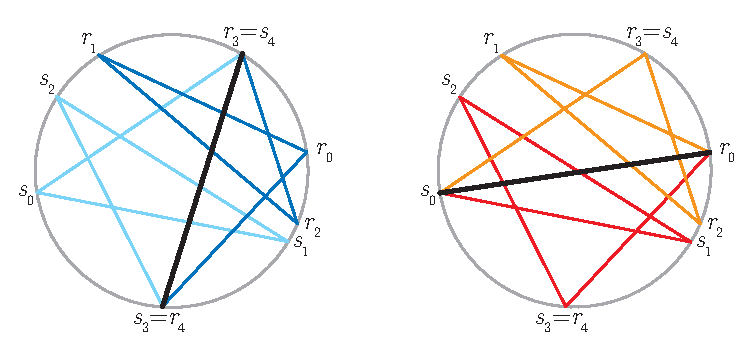
\includegraphics[scale=1]{flip.eps}}
\caption{\small{The flip of a $2$-relevant edge.}}\label{flip}
\end{figure}

We say that we obtain the $k$-triangulation $T\Delta\{e,f\}$ from the $k$-triangulation $T$ by \emph{flipping} the edge $e$. The $k$-triangulations $T$ and $T\Delta\{e,f\}$ are said to be \emph{flip-neighbours}. The added edge $f$ is denoted by $f(T,e)$.

\begin{bibremark}
This result is already proved in \cite{n-gdfcp-00} and \cite{j-gt}. But the proof is recursive and it does not permit to find explicitly the new edge. Note that this result is not proved in \cite{dkm-lahp-02}.

\end{bibremark}

Note that if $e$ is a $k$-relevant edge of a $k$-triangulation $T$ and $f=f(T,e)$, then $e$ and $f$ necessarily cross.
In particular, if $e=e_{\alpha\beta}$ and $f=e_{\gamma\delta}$ (with $0\le\alpha<\beta\le n-1$ and $0\le\gamma<\delta\le n-1$), then
\begin{itemize}
\item either $0\le\alpha<\gamma<\beta<\delta\le n-1$ and the flip is said to be \emph{slope-increasing},
\item or $0\le\gamma<\alpha<\delta<\beta\le n-1$ and the flip is said to be \emph{slope-decreasing}.
\end{itemize}
We define a partial order on the set of $k$-triangulations of the $n$-gon as follows: if $T$ and $T'$ are two $k$-triangulations of the $n$-gon, $T<T'$ if and only if there exists a sequence of slope-increasing flips from $T$ to $T'$ (if and only if there exists a sequence of slope-decreasing flips from $T'$ to $T$).
%DO WE HAVE TO EXPLAIN WHY IS IT ANTISYMETRIC ? (look at slopes)

Let $T_{n,k}^{\min}$ be the $k$-triangulation of the $n$-gon whose set of $k$-relevant edges is $\{e_{ij}\;|\;i\in\llbracket 0,k-1\rrbracket\;\mathrm{and}\;j\in\llbracket i+k,i-k\rrbracket\}$.

Let $G_{n,k}$ be the graph of flip-neighbours on the set of $k$-triangulations of the $n$-gon, ie. the graph whose vertices are the $k$-triangulations of the $n$-gon and whose edges are the pairs of flip-neighbour $k$-triangulations.

\begin{figure}
\centerline{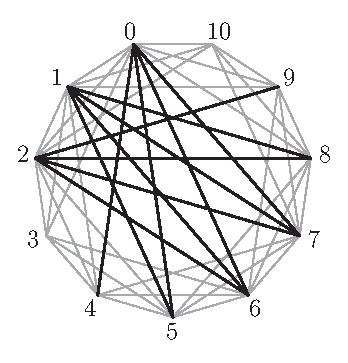
\includegraphics[scale=1]{min.eps}}
\caption{\small{The triangulation $T_{11,3}^{\min}$.}}\label{min}
\end{figure}

\begin{proposition}\label{connexity}
\begin{enumerate}
\item For any $k$-triangulation of the $n$-gon $T\ne T_{n,k}^{\min}$, there exists a $k$-relevant edge $e\in T\setminus T_{n,k}^{\min}$ such that $f(T,e)\in T_{n,k}^{\min}\setminus T$.
\item $T_{n,k}^{\min}$ is the least element of the set of $k$-triangulations of the $n$-gon partially ordered by $<$.
\item The graph $G_{n,k}$ is connected and its diameter is bounded by $2k(n-2k-1)$.
\end{enumerate}
\end{proposition}

\begin{proof}
Since the two last points are immediate corollaries of the first one, we only have to prove the first point.

Let $T$ be a $k$-triangulation of the $n$-gon distinct from $T_{n,k}^{min}$. Let
$$\ell=\max\{2k\le i\le n-k+1\;|\;[v_0,v_i],\ldots,[v_{k-1},v_{i+k-1}]\in T\},$$
which exists because $T\ne T_{n,k}^{min}$.

We claim that there exists $u\in\llbracket v_k, v_{\ell-2}\rrbracket$ such that $[u,v_{\ell+k-1}]$ is an edge of $T$. Indeed, suppose that this is not true and consider, for any $0\le j\le k-1$, the edge $f_j=[v_j,v_{\ell+j-1}]$. If $f_j$ is not in $T$, then $T$ contains a $k$-crossing preventing it.
Let $\{[x_1,y_1],\ldots,[x_k,y_k]\}$ denote this $k$-crossing, with the convention that
\begin{enumerate}[(i)]
\item $x_1<\ldots<x_k<y_1<\ldots<y_k$,
\item if $j>0$, $v_j\in\rrbracket x_j,x_{j+1}\llbracket$ and $v_{\ell+j-1}\in\rrbracket y_j,y_{j+1}\llbracket$,
\item if $j=0$ then $v_0\in\rrbracket y_k,x_1\llbracket$ and $v_{\ell+j-1}\in\rrbracket x_k,y_1\llbracket$.
\end{enumerate}
With this convention, we are sure that $x_k\in\llbracket v_k,v_{\ell-1}\rrbracket$ and $y_k\in\llbracket v_{\ell+k},v_{n-1}\rrbracket$. But then the set
$$\{[v_0,v_\ell],\ldots,[v_{k-1},v_{\ell+k-1}],[x_k,y_k]\}$$
is a $(k+1)$-crossing of $T$. This proves that for all $0\le j\le k-1$, the edge $[v_j,v_{\ell+j-1}]$ is in $T$ which contradicts the definition of $\ell$. So that the claim is proved.

Now let $m=\min\{k\le i\le \ell-2\;|\; [v_i,v_{\ell+k-1}]\in T\}$. Let $S$ be the $k$-star containing the edges $[v_{\ell+k-1},v_m]$ and $[v_{\ell+k-1},v_{k-1}]$ (theorem \ref{angle}) and let $R$ be the other $k$-star containing $[v_{\ell+k-1},v_m]$. Let $s_0, \ldots,s_{k-2},s_{k-1}=v_{k-1},s_k=v_m,s_{k+1},\ldots,s_{2k-1},s_{2k}=v_{\ell+k-1}$ denote the vertices of the $k$-star $S$ in circle order. Then $s_0\in\llbracket v_{\ell+k}, v_0\rrbracket$, and the only way not to get a $(k+1)$-crossing is to have $s_0=v_0$. And this implies that $s_j=v_j$ for all $0\le j\le k-1$. The following lemma concludes the proof.
\end{proof}

\begin{lemma}
Let $T$ be a $k$-triangulation. Let $S$ be a $k$-star of $T$ with vertices $s_0,\ldots, s_{2k}$ in cyclic order such that $s_0,\ldots,s_{k-1}$ are consecutive and $[s_k,s_{2k}]$ is a $k$-relevant edge. Let $R$ be the other $k$-star containing $[s_k,s_{2k}]$. Let $r$ and $s$ be the opposite vertices of $R$ and $S$. Then $s\in\{s_0,\ldots,s_{k-1}\}$.
\end{lemma}

\begin{proof}
The vertex $s$ can certainly not be $s_k$ or $s_{2k}$. And all the intervals $\rrbracket s_j,s_{j+1}\llbracket$, for $0\le j\le k-1$, are empty.
\end{proof}


\begin{remark}
\begin{enumerate}[(i)]
\item Note that the proposition \ref{connexity} gives an other proof of the number of edges (and consequently of $k$-stars) in a $k$-triangulation of the $n$-gon.
\item We get the same kind of results with the $k$-triangulation $T_{n,k}^{\max}$ whose set of $k$-relevant edges is $\{e_{ij}\;|\;i\in\llbracket n-k,n-1\rrbracket\;\mathrm{and}\;j\in\llbracket i+k,i-k\rrbracket\}$.
\end{enumerate}
\end{remark}

\begin{bibremark}
For $v\in V_n$ and $T$ a $k$-triangulation of the $n$-gon, let $d_v(T)$ denote the \emph{$k$-relevant degree} of $v$ in $T$, ie. the number of $k$-relevant edges of $T$ incident to $v$.
Let $\Upsilon(T)$ be the $n$-tuple $(d_{v_0}(T),\ldots,d_{v_{n-1}}(T))$.
Note that, \textsc{in contrast to what \cite{dkm-lahp-02} implicitly says}, the function $\Upsilon$ from $k$-triangulation of the $n$-gon to $\mathbb{N}^n$ is not injective (look for example for the two $2$-triangulations of the $8$-gon whose set of $2$-relevant edges are respectively $\{[1,4],[4,0],[0,5],[7,2],[2,6],[6,3]\}$ and $\{[1,6],[6,2],[2,5],[3,0],[0,4],[4,7]\})$. In particular, this does not give any linear order on the set of $k$-triangulations of the $n$-gon, and the argument of the paper is \textsc{absolutely wrong}.

The correct way to explain it is the following: the function $\Upsilon$ is a function, not necessarily injective, from the set of $k$-triangulations of the $n$-gon to the totally ordered set $\mathbb{N}^n$. But the minimum of this function is obviously reached uniquely for $T_{n,k}^{\min}$. Thus, since for any $k$-triangulation $T\ne T_{n,k}^{\min}$, there exists a flip-neighbour $T'$ of $T$ such that $\Upsilon(T')<\Upsilon(T)$, we are sure that the graph $G_{n,k}$ is connected.

Another way to say this is to consider the set of the $k$-triangulations of the $n$-gon partially ordered by the relation $T\ll T'$ if and only if $T=T'$ or $\Upsilon(T)<_{\mathrm{lex}}\Upsilon(T')$. This order is a refinement of the order $<$ defined above and $T_{n,k}^{\min}$ is the least element of the set of $k$-triangulations of the $n$-gon partially ordered by $\ll$.

Note that the paper \cite{dkm-lahp-02} does not prove that any $k$-relevant edge of a $k$-triangulation is flippable. Note that the paper \cite{n-gdfcp-00} proves that the diameter of $G_{n,k}$ is bounded by $(2k-4k^2/n)(n-2k-1)$. For all of these reasons, I believe that it is considerabily more preferable to look at \cite{n-gdfcp-00}.

\end{bibremark}


\section{Flattening a $k$-star, inflating a $k$-crossing}

Let $X_{n+1,k}$ be the Cartesian product of the set of $k$-triangulations of the $(n+1)$-gon and the set of $k$-almost-relevant edges of the $(n+1)$-gon.

Let $(T,e)\in X_{n,k}$ where $e=[s,s+k]$.
Let $s_0=s,s_1=s+1,\ldots,s_k=s+k,s_{k+1},\ldots,s_{2k}$ be the vertices of the unique $k$-star of $T$ containing $e$, in the circle order. Let $r_1,\ldots,r_k$ be $k$ points of the unit circle such that $s_0<r_1<s_1<r_2<\ldots<s_{k-1}<r_k<s_k$.

We name \emph{flattening} of $e$ in $T$ the set of edges $\underline{T}_e$ whose underlying set of points is the set $\{s+k+1,\ldots,s+n-1,r_1,\ldots,r_k\}$ and which is contructed from $T$ as follows (see fig. \ref{flatinfl}):
\begin{enumerate}[(i)]
\item for any edge of $T$ whose vertices are not in $\{s_0,\ldots,s_k\}$ just copy the edge.
\item forget all the edges of the complete graph on vertices $s_0,\ldots,s_k$, and add all the edges of the complete graph on vertices $r_1,\ldots,r_k$.
\item replace any edge of form $[s_i,t]$ with $0\le i\le k$, and $s+k+1\le t \le s_{k+i}$ (resp. $s_{k+i+1}\le t\le s-1$) by the edge $[r_i,t]$ (resp. $[r_{i+1},t]$).
\end{enumerate}
Let $E$ denote the $2k$-tuple $(r_1,\ldots,r_k,s_{k+1},\ldots,s_{2k})$ and define $$\Phi(T,e)=(\underline{T}_e,E).$$

\bigskip
Let $Y_{n,k}$ be the set of couples $(T,E)$ where $T$ is a $k$-triangulation of the $n$-gon and $E=(r_1,\ldots,r_k,s_{k+1},\ldots,s_{2k})$ is a $2k$-tuple of $V_{n}$ in cyclic order such that $r_k=r_1+k-1$ and $[r_i,r_{i+k}]$ is an edge of $T$ for all $1\le i\le k$.

Let $(T,E)\in Y_{n,k}$ where $E=(r_1,\ldots,r_k,s_{k+1},\ldots,s_{2k})$. Let $s_0,\ldots,s_k$ be $k+1$ points of the unit circle such that $r_1-1<s_0<r_1<s_1<\ldots<r_k<s_k<r_k+1$.

We name \emph{inflating} of $E$ in $T$ the set of edges $\overline{T}^E$ whose underlying set of points is the set $\{r_k+1,\ldots,r_1-1,s_0,\ldots,s_k\}$ and which is contructed from $T$ as follows (see fig. \ref{flatinfl}):
\begin{enumerate}[(i)]
\item for any edge of $T$ whose vertices are not in $\{r_1,\ldots,r_k\}$ just copy the edge.
\item forget all the edges of the complete graph on vertices $r_1,\ldots,r_k$, and add all the edges of the complete graph on vertices $s_0,\ldots,s_k$.
\item replace any edge of form $[r_i,t]$ with $1\le i\le k$, and $r_k+1\le t \le s_{k+i}$ (resp. $s_{k+i}\le t\le r_1-1$) by the edge $[s_i,t]$ (resp. $[s_{i-1},t]$).
\end{enumerate}
Let $e$ denote the edge $[s_0,s_k]$ and define $$\Psi(T,E)=(\overline{T}^E,e).$$

\begin{figure}
\centerline{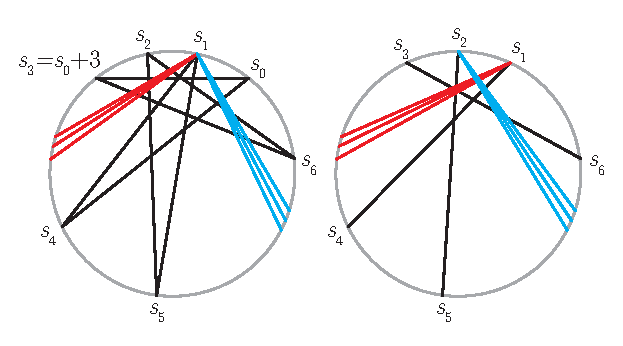
\includegraphics[scale=1]{flatinfl.eps}}
\caption{\small{Flattening a $3$-almost-relevant edge - inflating a $3$-crossing.}}\label{flatinfl}
\end{figure}

\begin{theorem}\label{flattening/inflating}
$\Phi$ and $\Psi$ define two inverse bijections between $X_{n+1,k}$ and $Y_{n,k}$.
\end{theorem}

\begin{proof} We first prove that the flattening of a $k$-triangulation of the $(n+1)$-gon is a $k$-triangulation of the $n$-gon. Consider the previous notations and note that:
\begin{enumerate}[(i)]
\item If $f$ is a $k$-relevant edge of $\underline{T}_e$, then
\begin{itemize}
\item either $f$ is of form $[r_i,s_{k+i}]$, for some $1\le i\le k$, and it corresponds to the two edges $f'=[s_{i-1},s_{k+i}]$ and $f''=[s_i,s_{k+i}]$ of the initial triangulation $T$,
\item or $f$ is not of the previous form, and it corresponds to a unique $k$-relevant edge $f'$ of $T$.
\end{itemize}
We deduce from this that $|\underline{T}_e|=|T|-2k$.

\item If $f$ and $g$ are two $k$-relevant edges of $\underline{T}_e$ and $f'$ and $g'$ are two $k$-relevant edges of $T$ that correspond to $f$ and $g$ respectively, then
\begin{itemize}
\item if $f$ and $g$ do not cross, then $f'$ and $g'$ do not cross,
\item if $f$ and $g$ do cross, then $f'$ and $g'$ do cross, except if there exists $i$ in $\{1,\ldots,k\}$, and $u,v$ two vertices such that $s+k<u\le s_{i+k}<s_{i+k+1}\le v<s$ and $f=[r_i,u]$, $g=[r_{i+1},v]$, $f'=[s_i,u]$ and $g'=[s_i,v]$. Such a configuration is said to be a \emph{hidden configuration}.
\end{itemize}

\end{enumerate}

The proof will now work in two steps: first prove that there is no $(k+1)$-crossing in $\underline{T}_e$, and then prove that we can not add any edge in $\underline{T}_e$ without creating a $(k+1)$-crossing.

\medskip
\noindent\textsc{First step.}
Let $F$ be a $(k+1)$-crossing of $\underline{T}_e$. We denote $f_1=[x_1,y_1],\ldots,f_{k+1}=[x_{k+1},y_{k+1}]$ the edges of $F$ ordered such that $x_1<x_2<\ldots<x_{k+1}<y_1<y_2<\ldots<y_{k+1}$. Let $f'_1=[x'_1,y'_1],\ldots,f'_{k+1}=[x'_{k+1},y'_{k+1}]$ denote $k$ edges of $T$ that correspond to the edges $f_1,\ldots,f_{k+1}$ respectively.

It is clear that if there exists no $1\le i\le k$ such that $(f_i,f_{i+1},f'_i,f'_{i+1})$ form a hidden configuration, then the edges $f'_1,\ldots,f'_{k+1}$ form a $(k+1)$-crossing of $T$, which is impossible. Thus we can suppose that the number of hidden configurations in the set $\{(f_i,f_{i+1},f'_i,f'_{i+1})\;|\; 1\le i\le k\}$ is at least $1$. We will find a new $(k+1)$-crossing $G$ of $\underline{T}_e$ and a set $G'$ of edges of $T$ that correspond to $G$ such that the number of hidden configurations in the set $\{(g_i,g_{i+1},g'_i,g'_{i+1})\;|\; 1\le i\le k\}$ is strictly less than in $\{(f_i,f_{i+1},f'_i,f'_{i+1})\;|\; 1\le i\le k\}$.

Let $i$ in $\{1,\ldots,k\}$ be such that $(f_i,f_{i+1},f'_i,f'_{i+1})$ is a hidden configuration. We can suppose that $x_i=r_i$ and $x_{i+1}=r_{i+1}$ (if this is not the case, we renumber the edges of $F$ such that this be true). Thus we know that $y_i\le s_{i+k}<s_{i+k+1}\le y_{i+1}$. Let $p$ denote the first integer before $i$ such that $x_p \ne r_p$ or $y_p>s_{p+k}$, and $q$ denote the first integer after $i+1$ such that $x_q \ne r_q$ or $y_q<s_{q+k}$.

Let $G$ be the set of $k+1$ edges of $\underline{T}_e$ deduced from $F$ as follows:
\begin{itemize}
\item for all $p<i<q$, let $g_i$ be $[r_i,s_{i+k}]$,
\item for all $q\le i\le p$, let $g_i$ be $f_i$.
\end{itemize}
Let $G'$ be the set of $k+1$ edges of $T$ constructed as follows:
\begin{itemize}
\item for all $p<i<q$, let $g'_i$ be $[s_i,s_{i+k}]$,
\item for all $q\le i\le p$, let $g'_i$ be $f'_i$.
\end{itemize}
		
It is quite clear that $G$ is a $(k+1)$-crossing of $\underline{T}_e$ and that $G'$ is a set of edges of $T$ that correspond to the edges of $G$. We just have to verify that the number of hidden configurations in the set $\{(g_i,g_{i+1},g'_i,g'_{i+1})\;|\; 1\le i\le k\}$ is less than in $\{(f_i,f_{i+1},f'_i,f'_{i+1})\;|\; 1\le i\le k\}$. But
\begin{enumerate}[(i)]
\item the number of hidden configurations in $\{(g_i,g_{i+1},g'_i,g'_{i+1})\;|\; q\le i<p\}$ is exactly the same as in $\{(f_i,f_{i+1},f'_i,f'_{i+1})\;|\; q\le i<p\}$,
\item there is no hidden configuration in $\{(g_i,g_{i+1},g'_i,g'_{i+1})\;|\; p<i<q-1\}$, whereas there is one hidden configuration in $\{(f_i,f_{i+1},f'_i,f'_{i+1})\;|\; p<i<q-1\}$,
\item the edges $(g_p,g_{p+1},g'_p,g'_{p+1})$ (resp. $(g_{q-1},g_q,g'_{q-1},g'_q)$) do not form a hidden configuration.
\end{enumerate}


\medskip
\noindent\textsc{Second step.}
We can use the fact that $|\underline{T}_e|=|T|-2k$ and the corollary \ref{starsenumeration}, or use a direct proof. Let $f$ be an edge that is not in $\underline{T}_e$. Let $f'$ be the unique edge that corresponds to $f$. Since $T$ is a $k$-triangulation, adding $f$ to $T$ creates a $(k+1)$-crossing $F'=\{f',f'_1,\ldots,f'_k\}$. Let $f_1,\ldots,f_k$ be the edges of $\underline{T}_e$ that correspond to $f'_1,\ldots,f'_k$ respectively. Then the set $F=\{f,f_1,\ldots,f_k\}$ forms a $(k+1)$-crossing of $\underline{T}_e$. This proves that we can not add any edge in $\underline{T}_e$ without creating a $(k+1)$-crossing and finishes the proof of the fact that the flattening of a $k$-triangulation of the $(n+1)$-gon is a $k$-triangulation of the $n$-gon.

\bigskip
We prove now that if $(T,E)\in Y_{n,k}$, then the inflating of $E$ in $T$ is a $k$-triangulation of the $(n+1)$-gon. Consider the previous notations and note that:
\begin{enumerate}[(i)]
\item If $f$ and $g$ are two $k$-relevant edges of $\overline{T}^E$ and $f'$ and $g'$ are the two edges of $T$ that correspond to $f$ and $g$ respectively, then if $f$ and $g$ do cross, then $f'$ and $g'$ do cross.
\item $|\overline{T}^E|=|T|+2k$.
\end{enumerate}

The proof is now immediate: (i) ensures that $\overline{T}^E$ does not present any $(k+1)$-crossing and (ii), combined with the corollary \ref{starsenumeration}, ensures that the number of edges of $\overline{T}^E$ is maximal.

\bigskip
The fact that $\Phi$ and $\Psi$ are inverse functions is obvious.
\end{proof}

\begin{bibremark}
This result is used in \cite{n-gdfcp-00} and \cite{j-gt} without speaking explicitly of stars.

\cite{e-btdp-06} uses the flattening in the very specific case when $k=2$ and the star we are flattening contains a $2$-ear. In this case, the proof that the flattening of a $2$-triangulation of the $(n+1)$-gon is a $2$-triangulation of the $n$-gon is obvious since there is no hidden configuration.

\end{bibremark}

\begin{remark}
\begin{enumerate}
\item Let $e$ and $f$ be two distinct $k$-almost-relevant edges of $T$. Let $e'$ (resp. $f'$) denote the corresponding edge of $e$ (resp. of $f$) in $\underline{T}_f$ (resp. $\underline{T}_e$). Then $e'$ (resp. $f'$) is a $k$-almost-relevant edge of $\underline{T}_f$ (resp. $\underline{T}_e$) and
$$\underline{\underline{T}_f}_{e'}=\underline{\underline{T}_e}_{f'},$$
so that we can speak of the flattening $\underline{T}_{A}$ of a set $A$ of $k$-almost-relevant edges of the $k$-triangulation $T$.

\item Let $(T,E)$ and $(T,F)$ be two elements of $Y_{n,k}$ such that the two $k$-crossing formed with $E$ and $F$ are disjoint. Then there exists a unique $E'$ such that $(\overline{T}^F,E')\in Y_{n+1,k}$ and the edges formed with  $E'$ correspond to the edges formed with $E$. Similary, there exists a unique $F'$ such that $(\overline{T}^E,F')\in Y_{n+1,k}$ and the edges formed with  $F'$ correspond to the edges formed with  $F$. Furthermore,
$$\overline{\overline{T}^F}^{E'}=\overline{\overline{T}^E}^{F'},$$
so that, if $B$ is a set such that for all $E\in B$, $(T,E)\in Y_{n,k}$ and for all $E\ne F\in B$, the two $k$-crossing formed with $E$ and $F$ are disjoint, then we can speak of the inflating $\overline{T}^B$ of $B$ in the $k$-triangulation $T$.

\item The proof of the theorem \ref{flattening/inflating} gives another proof of the number of $k$-stars (and consequently of edges) in a $k$-triangulation of the $n$-gon.
\end{enumerate}
\end{remark}

\begin{corollary}
Let $N(n,k)$ denote the number of $k$-triangulations of an $n$-gon. The quotient $N(n+1,k)/N(n,k)$ equals the average number of $k$-crossings on the first $k$ points among all $k$-triangulations of the $n$-gon.
\end{corollary}

\begin{remark}
For example,
\begin{enumerate}[(i)]
\item For $k=1$, we get that $N(n+1,1)/N(n,1)$ equals the average degree of vertex 1 in triangulations of the $n$-gon. Since the average degree of all triangulations of the $n$-gon is the same and equal to $(4n-6)/n$ we recover the well-known recursion for Catalan numbers:
\[
C_{n-1}=\frac{4n-6}{n}C_{n-2}.
\]

\item For $n=2k+1$ we have that $N(2k+1,k)=1$ (the unique $k$-triangulation is the complete graph)
and the number of $k$-crossings using the first $k$ vertices in this $k$-triangulation is $k+1$ (any choice of $k$ of the last $k+1$ vertices gives one $k$-crossing). In particular, we recover the fact that $N(2k+2,k)=k+1$.

\item Unfortunately, for $n>2k+1$ it is not true that the number of $k$-crossings using $k$ consecutive vertices is independent of the $k$-triangulation. Otherwise we would have that  $N(n+1,k)\cdot n /N(n,k)$ is an integer, equal to that number (as happens in the case of triangulations).
\end{enumerate}
\end{remark}



\section{Polygonal surface decomposition}

Any $k$-triangulation $T$ of the $n$-gon defines a polyhedral complex $\mathcal{C}(T)$ as follows:
\begin{enumerate}[(i)]
\item the vertices of $\mathcal{C}(T)$ are the vertices of the $n$-gon,
\item the edges of $\mathcal{C}(T)$ are the $k$-almost-relevant edges and $k$-relevant edges of $T$,
\item the facets of $\mathcal{C}(T)$ are the $k$-stars of $T$.
\end{enumerate}
The number of vertices (resp. edges, resp. facets) of $\mathcal{C}(T)$ is $n$ (resp. $k(n-2k-1)+n$, resp. $n-2k$), and we can view the polyhedral complex $\mathcal{C}(T)$ as a decomposition into $(2k+1)$-gons of a surface $\mathcal{S}_{n,k}$ with $\gcd(n,k)$ boundaries and of genus
$$g_{n,k}=\frac{1}{2}(2-f+e-v-b)=\frac{1}{2}(2-n+k+kn-2k^2-\gcd(n,k)).$$

\begin{remark}
Let $T$ be a $k$-triangulation of the $n$-gon, and let $e$ be a $k$-relevant edge of $E$. Let $R$ and $S$ be the two $k$-stars of $T$ containing $e$, let $r$ and $s$ be the opposite vertices of $R$ and $S$, and let $f=[r,s]$. Let $X$ and $Y$ be the two $k$-stars of $T\Delta\{e,f\}$ containing $f$.

Then $T\setminus\{e\}$ can be viewed as a decomposition of $\mathcal{S}_{n,k}$ into $n-2k-2$ $(2k+1)$-gons and one $(4k)$-gon, obtained from $\mathcal{C}(T)$ by gluing the two $(2k+1)$-gons corresponding to $R$ and $S$ along the edge $e$. And then $T\Delta\{e,f\}$ is obtained from $T\setminus\{e\}$ by splitting the $(4k)$-gon into the two $(2k+1)$-gons corresponding to $X$ and $Y$.
\end{remark}

The end of this section is devoted to an application of this point of view to regular polygonal decompositions of surfaces of high genus.

Assume that $k$ is even and $n=2(2k+1)$. A \emph{$k$-zigzag} of $E_{2(2k+1)}$ is a subset of $k$-relevant edges of the form
$$Z_\gamma^+=\{[\gamma-p,\gamma+k+p+1]\;|\; 0\le p\le k\}\cup\{[\gamma-p-1,\gamma+k+p+1]\;|\; 0\le p\le k-1\}$$
or of the form
$$Z_\gamma^-=\{[\gamma+p,\gamma-k-p-1]\;|\; 0\le p\le k\}\cup\{[\gamma+p+1,\gamma-k-p-1]\;|\; 0\le p\le k-1\},$$
where $\gamma\in\mathbb{Z}_{2(2k+1)}$.

\begin{figure}
\centerline{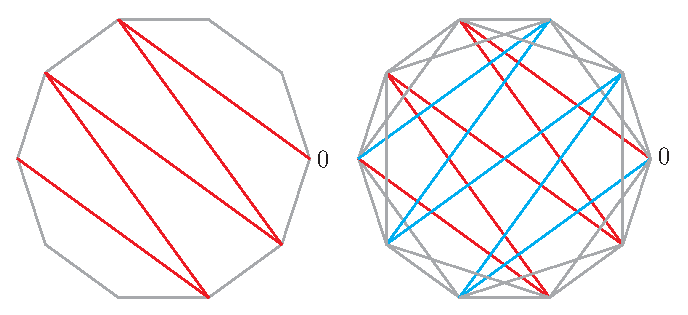
\includegraphics[scale=1]{10-gon.eps}}
\caption{\small{The $2$-zigzag $Z_0^+$ (left) and the $2$-triangulation $T_2$ (right).}}\label{10-gon}
\end{figure}


\begin{lemma}
The set
$$\bigcup_{\gamma=0}^{k/2-1} (Z_{2\gamma}^+\cup Z_{2\gamma}^-)$$
is the subset of the $k$-relevant edges of a $k$-triangulation $T_k$ of the $2(2k+1)$-gon.
\end{lemma}

\begin{proof}
Since there is no $2$-crossing in a $k$-zigzag, there is no $(k+1)$-crossing in the union of $k$ $k$-zigzags. Moreover, a $k$-zigzag contains $2k+1$ $k$-relevant edges so that the disjoint union of $k$ $k$-zigzags contains $k(2k+1)=k(2(2k+1)-2k-1)$ $k$-relevant edges. The corollary \ref{starsenumeration} ensures that we get a $k$-triangulation $T_k$ of the $2(2k+1)$-gon.
\end{proof}

\begin{lemma}\label{transformation}
The triangulation $T_k$ is invariant by the rotation $\rho: t\mapsto t+2k+1$ and by the symmetry $\delta: t\mapsto k/2-1-t$.
\end{lemma}

\begin{proof}
Any $k$-zigzag is invariant by the rotation $\rho$ so that the union of $k$-zigzags is invariant by $\rho$.

For any $0\le\gamma\le k/2-1$, $\delta(Z^+_{2\gamma})=Z^-_{2(k/2-1-\gamma)}$ and $\delta(Z^-_{2\gamma})=Z^+_{2(k/2-1-\gamma)}$ so that $T_k$ is invariant by $\delta$.
\end{proof}

\begin{lemma}
The degree of any vertex $v$ in the triangulation $T_k$ is $3k$.
\end{lemma}

\begin{proof}
Let $u$ and $v$ be two vertices of $V_{2(2k+1)}$. Then
\begin{itemize}
\item If $u=v$ or $u=v+2k+1$, then $v$ is adjacent to one edge of $Z_u^+$ and one edge of $Z_u^-$.
\item If $v\in\llbracket u+1,u+k\rrbracket$ or $v\in\llbracket u+2k+2,u+3k+1\rrbracket$ then $v$ is adjacent to two edges of $Z_u^-$ and is not adjacent with $Z_u^+$.
\item If $v\in\llbracket u+k+1,u+2k\rrbracket$ or $v\in\llbracket u+3k+2,u-1\rrbracket$ then $v$ is adjacent to two edges of $Z_u^+$ and is not adjacent with $Z_u^-$.
\end{itemize}
In particular, $v$ is adjacent with exactly two edges of $Z_u^+\cup Z_u^-$. This proves that the vertex-degree in $T_k$ is constant and equals $2.k/2+2k=3k$.
\end{proof}

Now we need a description of the $k$-stars of $T_k$. For any $0\le\gamma\le k/2-1$, let $s_\gamma:\mathbb{Z}_{2k+1}\to V_{2(2k+1)}$ denote the function defined by
$$s_{\gamma}(i)=\left\{\begin{array}{ll}
2\gamma+i  &  \mathrm{if}\;0\le i< k+2 \\
2\gamma+3i-2k-3  &  \mathrm{if}\;k+2\le i< 3k/2+1-\gamma \\
2\gamma+3i-2k-2  &  \mathrm{if}\;3k/2+1-\gamma\le i< 2k+1-\gamma \\
2\gamma+3i-2k-1  &  \mathrm{if}\;2k+1-\gamma\le i< 2k+1.
\end{array}\right.$$
Let $x:\mathbb{Z}_{2k+1}\to V_{2(2k+1)}$ be defined by
$$x(i)=\left\{\begin{array}{ll}
i-1  &  \mathrm{if}\;0\le i< k+1 \\
3i-2k-2  &  \mathrm{if}\;k+1\le i< 3k/2+1 \\
3i-2k-1  &  \mathrm{if}\;3k/2+1\le i< 2k+1.
\end{array}\right.$$

\begin{lemma}
\begin{enumerate}
\item For any $0\le\gamma\le k/2-1$, the set $\{s_{\gamma}(i)\;|\; i\in\mathbb{Z}_{2k+1}\}$ is the set of the vertices of a $k$-star $S_{\gamma}$ of $T_k$.
\item The set $\{x(i)\;|\; i\in\mathbb{Z}_{2k+1}\}$ is the set of the vertices of a $k$-star $X$ of $T_k$.
\item The set of $k$-stars of $T_k$ is the set
$$\{X,\rho(X)\}\cup\bigcup_{\gamma=0}^{k/2-1}\{S_{\gamma}, \rho(S_{\gamma}),\delta(S_{\gamma}),\rho\circ\delta(S_{\gamma})\}.$$
\end{enumerate}
\end{lemma}

\begin{proof}
Let $k+2\le i< 3k/2+1-\gamma$, $\lambda=2(\gamma+i-k-1)$ and $p=i-k-2$. Then
$$\lambda-p=2\gamma+i-k=s_{\gamma}(i-k),$$
$$\lambda-p-1=s_{\gamma}(i-k-1),$$
$$\mathrm{and}\; \lambda+k+p+1=2\gamma+3i-2k-3=s_\gamma(i).$$
This proves that the edges $[s_{\gamma}(i-k),s_\gamma(i)]$ and $[s_{\gamma}(i-k-1),s_{\gamma}(i)]$ are edges of the $k$-zigzag $Z^+_{\lambda}\subset T_k$.

Similarily, for any $3k/2+1-\gamma\le i< 2k+1-\gamma$, the edges $[s_{\gamma}(i-k),s_\gamma(i)]$ and $[s_{\gamma}(i-k-1),s_\gamma(i)]$ are edges of the $k$-zigzag $Z^-_{2(i-3k/2-1+\gamma)}\subset T_k$ and for any $2k+1-\gamma\le i< 2k+1$, the edges $[s_{\gamma}(i-k),s_\gamma(i)]$ and $[s_{\gamma}(i-k-1),s_\gamma(i)]$ are edges of the $k$-zigzag $Z^+_{2(i-2k-1+\gamma)}\subset T_k$. Furthermore, the edge $[s_\gamma(0),s_{\gamma}(k+1)]$ is in $Z^+_{2\gamma}\subset T_k$ and the edges $[s_\gamma(0),s_{\gamma}(k)]$ and $[s_\gamma(1),s_{\gamma}(k+1)]$ are $k$-almost-relevant. Thus we have proved that the $2k+1$ edges joining the points of $\{s_{\gamma}(i)\;|\; i\in\mathbb{Z}_{2k+1}\}$ in star order are edges of $T_k$ which proves that this set is the set of vertices of a $k$-star $S_{\gamma}$.


\bigskip
Similarily, we prove that for any $k+1\le i< 3k/2+1$, the edges $[x(i-k),x(i)]$ and $[x(i-k-1),x(i)]$ are edges of the $k$-zigzag $Z^+_{2(i-k-1)}\subset T_k$ and for any $3k/2+1\le i< 2k+1$, the edges $[x(i-k),x(i)]$ and $[x(i-k-1),x(i)]$ are edges of the $k$-zigzag $Z^-_{2(i-3k/2-1)}\subset T_k$. Since $[x(0),x(k)]$ is $k$-almost-relevant, the $2k+1$ edges joining the points of $\{x(i)\;|\; i\in\mathbb{Z}_{2k+1}\}$ in star order are edges of $T_k$, and thus this set is the set of vertices of a $k$-star $X$.

\bigskip
Finally, by lemma \ref{transformation}, $\rho(X)$ and $\rho(S_\gamma)$, $\delta(S_\gamma)$ and $\rho\circ\delta(S_\gamma)$ (for $0\le\gamma\le k/2-1$) are $k$-stars of $T_k$. The following lemma will ensure that all these $k$-stars are distinct. In particular, we get all the $2k+2$ $k$-stars of $T_k$ (lemma \ref{starsenumeration}), which proves the last point.
\end{proof}

\begin{figure}
\centerline{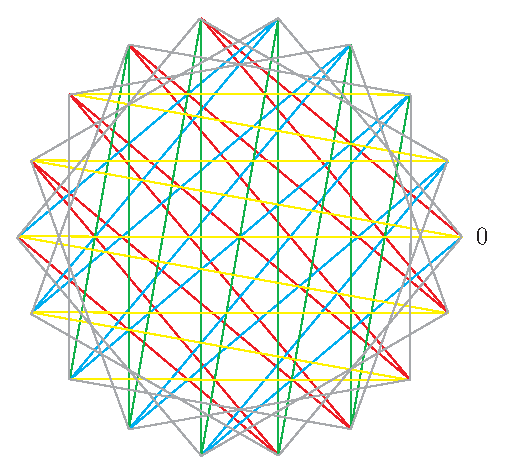
\includegraphics[scale=1]{18-gon.eps}}
\caption{\small{The $4$-triangulation $T_4$ (the $4$-irrelevant edges have been deleted).}}\label{18-gon}
\end{figure}

\begin{lemma}
The edge $[x(0),x(k)]=[-1,k-1]$ is the only $k$-almost-relevant edge of the $k$-star $X$. For any $0\le\gamma\le k/2-1$, the edges $[s_\gamma(0),s_{\gamma}(k)]=[2\gamma,2\gamma+k]$ and $[s_\gamma(1),s_{\gamma}(k+1)]=[2\gamma+1,2\gamma+k+1]$ are the only two $k$-almost-relevant edges of the $k$-star $S_\gamma$.
\end{lemma}

\begin{proof}
Note that if $r_0,\ldots,r_{2k}$ are the vertices of a $k$-star, in circle order, then the edge $[r_i,r_{i+k}]$ is $k$-almost-relevant if and only if the vertices $r_i,r_{i+1},\ldots, r_{i+k}$ are consecutive. The definitions of $x$ and $s_\gamma$ thus give the above result.
\end{proof}

\begin{lemma}
Any pair $\{R,S\}$ of $k$-stars of $T_k$ shares at most one edge. More precisely,
\begin{enumerate}
\item Any pair $\{R,S\}$ of $k$-stars of $T_k$ such that $S\notin\{\delta(R),\rho(R),\delta\circ\rho(R)\}$ shares exactly one edge,
\item For any $0\le\gamma\le k/2-1$, $\{S_\gamma,\rho(S_\gamma)\}$ shares exactly one edge and $\{S_\gamma,\delta(S_\gamma)\}$ (resp. $\{S_\gamma,\rho\circ\delta(S_\gamma)\}$) does not share any edge,
\item $\{X,\rho(X)\}$ does not share any edge.
\end{enumerate}
\end{lemma}

\begin{proof}
Let $0\le\gamma\le k/2-1$.
If $\gamma$ is even, then
\begin{eqnarray*}
s_{\gamma}(-\gamma/2)&=&2\gamma+3(2k+1-\gamma/2)-2k-1\\
&=&\gamma/2+2(2k+1)\equiv \gamma/2=x(\gamma/2+1),\\
\mathrm{and}\;s_{\gamma}(k+1-\gamma/2)&=&2\gamma+(k+1-\gamma/2)=3\gamma/2+k+1\\
&=&3(\gamma/2+k+1)-2k-2=x(\gamma/2+k+1).
\end{eqnarray*}
so that the edge $[\gamma/2,3\gamma/2+k+1]$ is common to $S_\gamma$ and $X$.
Similarily, we prove that:
\begin{enumerate}
\item If $\gamma$ is odd, then $[\gamma/2-3/2,3\gamma/2+k+1/2]\in S_\gamma\cap X$.
\item If $\gamma$ is even, then $[3\gamma/2+5k/2+2,\gamma/2+k/2]\in\rho(S_\gamma)\cap X$.
\item If $\gamma$ is odd, then $[3\gamma/2+5k/2+1/2,\gamma/2+k/2-3/2]\in\rho(S_\gamma)\cap X$.
\end{enumerate}
Since $X$ is invariant by the symmetry $\delta$, this proves that for any $0\le\gamma\le k/2-1$,
$S_\gamma\cap X\ne\emptyset$, $\rho(S_\gamma)\cap X\ne\emptyset$, $\delta(S_\gamma)\cap X\ne\emptyset$ and $\rho\circ\delta(S_\gamma)\cap X\ne\emptyset$.
But the $k$-star $X$ contains one $k$-almost-relevant edge and $2k$ $k$-relevant edges so that we get
$$|S_\gamma\cap X|=|\rho(S_\gamma)\cap X|=|\delta(S_\gamma)\cap X|=|\rho\circ\delta(S_\gamma)\cap X|=1$$
$\mathrm{and}\; X\cap\rho(X)=\emptyset$. The invariance by rotation ensures the same result for $\rho(X)$.

For any $0\le\gamma<\gamma'\le k/2-1$, we prove with the same method that $S_\gamma\cap S_{\gamma'}\ne\emptyset$, $S_\gamma\cap \delta(S_{\gamma'})\ne\emptyset$, $S_\gamma\cap \rho(S_{\gamma'})\ne\emptyset$ and $S_\gamma\cap \rho\circ\delta(S_{\gamma'})\ne\emptyset$.
Furthermore, for any $0\le\gamma\le k/2-1$, $[2\gamma+k/2,2\gamma+5k/2+1]\in S_\gamma\cap \rho(S_{\gamma})$. The fact that $S_\gamma$ contains $2k-1$ $k$-relevant edges ensures that $S_\gamma$ shares exactly one edge with $X$, $\rho(X)$, $\rho(S_\gamma)$ and $S_{\gamma'}$, $\delta(S_{\gamma'})$, $\rho(S_{\gamma'})$ and $\rho\circ\delta(S_{\gamma'})$ (for any $0\le\gamma\le k/2-1$ distinct from $\gamma$) which finishes the proof.
\end{proof}

Let $X$ and $Y$ be two $(2k+1)$-gons with respective set of edges $\{[2i,2i+k]\;|\; 0\le i\le 2k\}$ and $\{[2i+1,2i+1+k]\;|\; 0\le i\le 2k\}$ and let $\hat{\mathcal{C}}_k$ denote the polyhedral complex $\mathcal{C}(T_k)\cup\{X,Y\}$.
Let $\mathcal{U}_k$ denote a closed surface of genus $g_k=k^2-\frac{k}{2}-1$.

With the four previous lemmas, we get:

\begin{corollary}
The polyhedral complex $\hat{\mathcal{C}}_k$ forms a decomposition of $\mathcal{U}_k$ into $(2k+1)$-gons with $2(2k+1)$ vertices, $(2k+1)(k+2)$ edges and $2(k+2)$ polygons, such that
\begin{enumerate}
\item all the vertices have the same degree $k+2$,
\item two $(2k+1)$-gons do not share more than one edge (the decomposition is regular).
\end{enumerate}
\end{corollary}




\section{Multi-Dick-paths}

IN PROGRESS


\section{Multi-associahedron}

IN PROGRESS

\bibliographystyle{alpha}
\bibliography{biblio.bib}




\end{document}
